\section{Design and Implementation}
\label{sec-design}
Our goal is to build a file system for a tiered storage hierarchy consisting of disks and NVM that combines the low latency of NVM and low cost of disk-based storage without regressing on performance while offering similar consistency guarantees as BPFS. Our goal is to extend BPFS to build a file system spanning NVM and disks. To build such a file system, here are a set of policies and mechanisms we need to come up with.

\begin{itemize}
\item A mechanism that supports moving data between persistent memory and disks. How do we make changes to BPFS data structures so that we can locate the data in memory or disk?
\item Do we handle disks directly or do we go through another file system to store data on disk?
\item What is the ideal granularity at which we move the data? 
\item What policies determine when to move data?
\end{itemize}

Figure~\ref{fig-bpfs} depicts the overall design of our system. We use NVM to store the meta data and hot data blocks and push the cold data blocks to disk. We have made changes to the indirect pointer in the BPFS tree depicted in Figure~\ref{fig-bpfstree} and use the most significant bit to locate the data between persistent memory and disk. Disk manager transparently manages the disk and gives logical addresses for the cold data blocks on disk. We describe disk manager and anti-caching manager in the following subsections.

\subsection{Anti-Cache Manager}
Non Volatile Memory (NVM) is the primary data store and it also contains the more frequently accessed blocks, which is referred to as hot data. But since the capacity of the persistent NVM is limited, we have used the concept of Anti-Caching to periodically evict blocks from the NVM to the disk periodically based on an eviction policy. The eviction policy thus used in this design is the Least Recently Used (LRU) policy. The Anti-Cache Manager keeps track of all the blocks that are written to the NVM and periodically evicts blocks when the number of blocks in the NVM exceeds a pre-determined threshold, which is used to ensure that the NVM is always available from writing blocks, which has helped us drastically reduce our write latency for blocks.

\begin{figure}
\centering
\vspace{-0.2in}
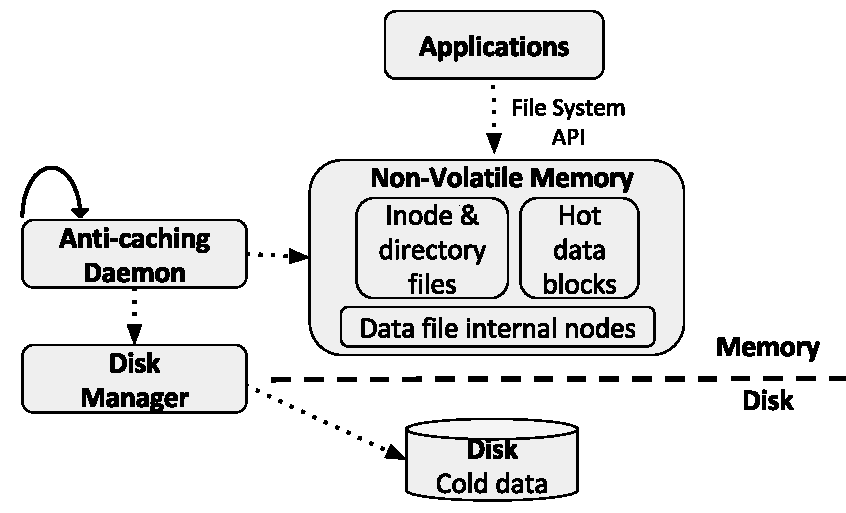
\includegraphics[width=0.5\textwidth]{figs/bpfs.pdf}
\vspace{-0.2in}
\mycaption{fig-bpfs}{Design Overview of BPFS}{\footnotesize The figure shows the overall design of our system.}
\end{figure}

In order to achieve this, the anti-cache manager runs as a separate background thread that continuously probes the NVM and performs silent eviction. In order to ensure that data blocks that are currently being evicted to disk do not get updated by the file system, a block level locking mechanism is used which implicitly prevents any updates to the block currently being evicted. 

\subsection{Disk Manager}
The Disk Manager component simulates a virtual disk using a file stored on disk in the BPFS partition of a predetermined size. It exposes APIs for reading and writing blocks into the disk individually and in bulk. It performs prefetching of additional blocks when a read is performed. The lifetime of the prefetched blocks in memory is predetermined to ensure that unused prefetched blocks are cleaned up regularly with the help of a background thread. To avoid fragmentation, a free list of blocks that have been freed is maintained. Since the disk manager writes blocks to a file, the buffer cache is used to buffer writes until all the blocks are written into the file. Our current implementation provides consistency at the expense of performance by notifying BPFS after persisting the blocks, which inturn updates the indirect pointer in the inodes to point to the new blocks through a blocking call.

The disk manager also exposes another write API to the Anti-Cache Manager to facilitate writing one block at a time, for faster random writes since any free block on disk can be used for writing and does not require sequential locality. To further improve performance in the case of bulk eviction of blocks from the anti-cache manager, the disk manager performs an explicit flush only after writing all the blocks on to the disk.

\begin{figure}
\centering
\vspace{-0.2in}
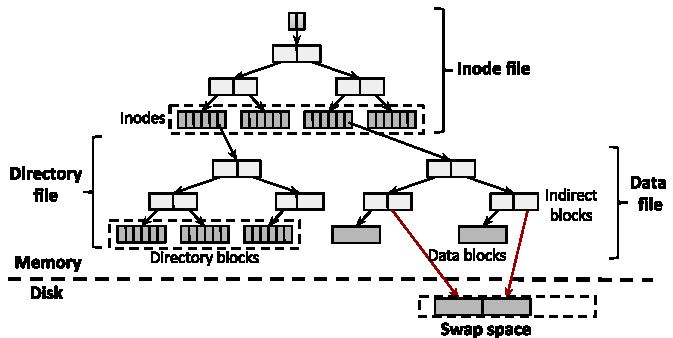
\includegraphics[width=0.5\textwidth]{figs/bpfs2.pdf}
\vspace{-0.2in}
\mycaption{fig-bpfstree}{BPFS tree structure}{\footnotesize The figure shows the file system organization of our modified BPFS}
\end{figure}

\subsection{File System Operations}
In this section we describe the workflows for various file system operations.
\subsubsection{Read}
When a read operation is performed on a file, the BPFS crawls the inode tree to the indirect block containing the pointer to the data block, identifies the location of the data block using the MSB that indicates whether the block is on disk or in NVM, then fetches the block into memory and asynchronously writes it back into NVM. Once the block is persisted in NVM, it frees the block on disk and updates the indirect pointer in the inode tree to point to the new block location in NVM atomically.

When a read operation is performed on a directory, the BPFS crawls the inode tree and the directory file blocks are loaded into memory from NVM and the necessary updates are made into the directory entry cache. It then traverses all the necessary inodes in the directory file and reads them from NVM.
 
\subsubsection{Write}
When a write operation is performed on a file, the BPFS traverses the inode tree to find the indirect block containing the pointers to the data block of the file and identifies the location of the data blocks. If the data block is in NVM, the write operation is performed in-place and has no additional overhead. If the data block is on disk, the block is fetched into NVM thus performing a copy on write of the data block and this block is updated and written back to NVM. The block on disk is then freed and the control comes back to the BPFS crawler. The indirect pointer in the inode tree is then updated to point to this new block location in-place along with in-place writes of the other internal nodes. The inode access time is also updated through an in-place atomic write.

\subsubsection{Open}
When a file is opened, the directory inode tree is parsed to find the file. If the file is not found and a create is requested, a new inode number is generated and the new inode is written to the inode file. Then the directory file is then updated. All these updates are performed in place. Since the metadata updates are in-place and in NVM, they are faster than usual disk writes and the additional overhead of metadata journaling can also be avoided by avoiding disk writes.
